\documentclass{article}
\usepackage[utf8]{inputenc}

\title{Pesquisa Operacional - Relatório 09}
\author{Adriel Cardoso dos Santos}
\date{Maio 2018}
\usepackage{amsmath}
\usepackage{amssymb}
\usepackage[]{algorithm2e}
\usepackage{graphicx}
\begin{document}

    \maketitle

    \section{Descrição do problema}

    Foi pedido a implemetação de um modelo que solucionasse o problema do caxeiro viajante utilizando programação linear.

    \section{Modelo}

    \subsection{Variáveis de decisão}
    \begin{enumerate}
        \item $E_i_j \in \{0, 1\}$, representando se a aresta do nó $i$ ao nó $j$ está ativada.
    \end{enumerate}
    \subsection{Variáveis auxiliares}
    \begin{enumerate}
        \item $d_i_j \in {\rm I\!R}$, representando a distância do nó $i$ ao nó $j$.
    \end{enumerate}


    \subsection{Restrições}
    \subsubsection{Restrição de Linhas}
    Só se deve partir uma aresta de cada nó, dessa forma a utilizo a equação (1) para determinar essa restrição.
    \begin{equation}
        \sum_{j = 0}^{k} E_i_j = 1 \quad
        \forall i=1..n
    \end{equation}

    \subsubsection{Restrição de Colunas}
    Cada nó deve receber apenas uma aresta, a equação (2) define essa restrição.
    \begin{equation}
        \sum_{i = 0}^{k} E_i_j = 1 \quad
        \forall j=1..n
    \end{equation}

    \subsubsection{Restrição de loops}
    O programa faz chamadas ao solver iterativamente a cada solução gerada, procura-se por loops que não contemplem todos os nós do grafo, caso um
    desses loops seja encontrado esse loop deve ser removido do modelo, adicionando uma restrição.


    \subsection{Função objetivo}
    A equação (3) define a função objetivo do modelo.
    \begin{equation}
        \sum_{i = 0}^{k} \sum_{j = 0}^{k} E_i_j d_i_j \quad
    \end{equation}

    \section{Conclusão}
    Foi possível solucionar o problema do caxeiro viajante rapidamente na sua otimalidade para a instância de 10 vertices.
    Para as outras instâncias não foi possível obter uma solução em tempo viável.
    É possível ver o grafo de resultado para a instância de 10 vertices na figura~\ref{fig:Grafo}

    \begin{figure}
        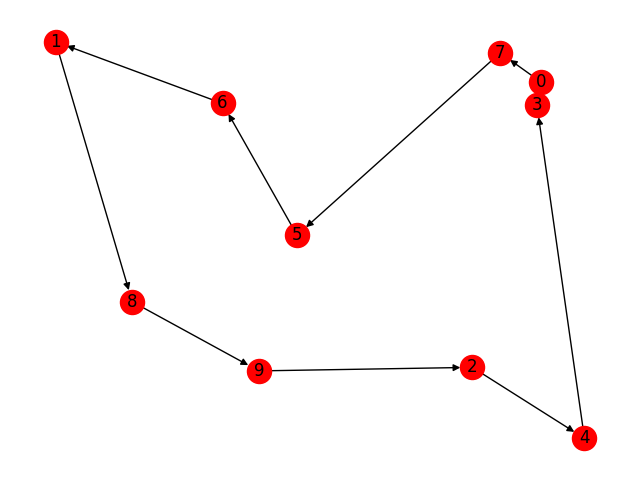
\includegraphics[width=\linewidth]{res_10.png}
        \caption{Resultado para instância de 10 vertices.}
        \label{fig:Grafo}
    \end{figure}

\end{document}